\documentclass[11pt,a4paper]{article}

% ====================================================================
%  Introduccion a Bases de Datos (IBD) - UBA 2026
%  Trabajo Practico Grupal - Informe condensado
%  Replica en LaTeX de INFORME_CONDENSADO.md
% ====================================================================

\usepackage[utf8]{inputenc}
\usepackage[T1]{fontenc}
\usepackage[spanish,es-noindentfirst]{babel}
\usepackage{lmodern}
\usepackage[margin=2.3cm]{geometry}
\usepackage{graphicx}
\usepackage{booktabs}
\usepackage{array}
\usepackage{longtable}
\usepackage{enumitem}
\usepackage{xcolor}
\usepackage{listings}
\usepackage{amsmath}
\usepackage{hyperref}
\usepackage{caption}

% --- Numeracion de tablas como "Tabla" (babel usa "Cuadro" por defecto) -------
\addto\captionsspanish{\renewcommand{\tablename}{Tabla}}

% --- Estilo de hipervinculos -------------------------------------------------
\hypersetup{
    colorlinks=true,
    linkcolor=blue!55!black,
    urlcolor=blue!55!black,
    citecolor=blue!55!black,
    pdftitle={Introduccion a Bases de Datos - Trabajo Practico Grupal},
    pdfauthor={Teo Nabot, Mario Sigal, Felipe Pasquet}
}

% --- Ruta de imagenes --------------------------------------------------------
\graphicspath{{img_informe/}}

% --- Estilo para fragmentos de codigo/SQL ------------------------------------
\definecolor{codebg}{rgb}{0.96,0.96,0.96}
\lstset{
    basicstyle=\ttfamily\small,
    backgroundcolor=\color{codebg},
    breaklines=true,
    frame=single,
    framesep=4pt,
    rulecolor=\color{gray!40},
    columns=fullflexible,
    keepspaces=true,
    showstringspaces=false,
    aboveskip=8pt,
    belowskip=8pt
}

% --- Notas de captura (placeholders del original) ----------------------------
\newcommand{\captura}[1]{%
    \par\vspace{4pt}%
    \noindent\fcolorbox{gray!50}{gray!8}{%
        \parbox{0.97\linewidth}{\small\itshape\faintnote{}#1}%
    }\par\vspace{4pt}%
}
\newcommand{\faintnote}{\textbf{[captura]}~}

\title{\vspace{-1.5cm}\textbf{Introducción a Bases de Datos (IBD)}\\[0.4em]
       \Large Trabajo Práctico Grupal}
\author{Teo Nabot (LU: 996/22) \and Mario Sigal (LU: 157/22) \and Felipe Pasquet (LU: 1084/22)}
\date{}

\begin{document}

\maketitle
\thispagestyle{empty}

\tableofcontents
\vspace{1em}
\hrule
\vspace{1em}

% ============================================================================
\section{Etapa 1 — Modelo Relacional (PostgreSQL)}
% ============================================================================

\subsection{Elección del Modelo}

\subsubsection*{Dominio elegido y su relevancia}

Se modeló el \textbf{comercio minorista de suplementos deportivos}: una cadena con
varias sucursales que compra productos a proveedores, mantiene stock por sucursal y
los vende a clientes.

Se eligió este dominio porque es suficientemente rico para sustentar todas las etapas
del TP y porque se trata de un negocio real que nos podemos comunicar con el dueño para
hacer preguntas específicas del dominio y además ya existe un modelado básico del
problema. Incluye relaciones de distintas cardinalidades y opcionalidades, genera
\textbf{métricas de negocio reales} (facturación, profit, ticket promedio, rotación de
stock, recencia/frecuencia de clientes), permite consultas complejas uniendo distintas
entidades y también admite \textbf{nuevos requerimientos} naturales (ventas online con
cola de despacho, combos de productos, estado actual de stock consultado en tiempo real)
que motivan la persistencia políglota de la Etapa 4.

\subsubsection*{Decisiones de diseño}

Además de incluir las entidades fundamentales para modelar el dominio elegido
(\texttt{PRODUCTOS}, \texttt{CLIENTES}, \texttt{VENTAS}, \texttt{COMPRAS},
\texttt{PUNTOS\_DE\_VENTA}, \texttt{PROVEEDORES}) decidimos incluir la relación
\texttt{STOCK} como tabla asociativa M:N entre \texttt{PRODUCTOS} y
\texttt{PUNTOS\_DE\_VENTA}, con clave primaria compuesta
(\texttt{product\_id}, \texttt{puntos\_de\_venta\_id}). Además, en compras y ventas,
incluimos \texttt{DETALLE\_VENTAS} y \texttt{DETALLE\_COMPRAS}.
\texttt{COMPRAS}/\texttt{VENTAS} guardan los datos comunes de la transacción (fecha,
punto de venta, método de pago) y el detalle, una fila por producto, así evitamos
repetir los datos de cabecera en cada línea.

Para poder modelar costos cambiantes en los productos, modelamos el costo del producto
con \texttt{ultimo\_costo}: representa el último costo de reposición conocido.

\begin{figure}[ht]
    \centering
    \includegraphics[width=0.5\linewidth]{der viejo.jpeg}
    \includegraphics[width=0.49\linewidth]{der final.png}
    \caption{Diagramas Entidad-Relación: modelo original (izquierda) vs. modelo final
    (derecha), reflejando las decisiones de diseño tomadas. Versiones de mayor nitidez
    en el anexo.}
    \label{fig:der}
\end{figure}

Luego, en \texttt{DETALLE\_VENTAS}, el \texttt{costo\_unidad} representa el valor de
\texttt{ultimo\_costo} de ese producto en el momento de la venta. Así logramos modelar
que ventas distintas del mismo producto tengan costos distintos a lo largo del tiempo.

También decidimos modelar el \textbf{método de pago como entidad propia}
(\texttt{METODOS\_PAGO}, referenciada por \texttt{VENTAS.metodo\_pago\_id}) en lugar de un
atributo \texttt{ENUM}/\texttt{CHECK IN (...)}. Esto permite agregar o renombrar medios de
pago sin alterar la tabla \texttt{VENTAS} y evita un dominio rígido embebido en el esquema.

\textbf{Dejamos afuera} todos los \textbf{atributos derivables (decisión de
normalización):} no se almacena nada que pueda calcularse a partir de otras columnas
para evitar redundancia. Se eliminaron \texttt{subtotal} y \texttt{profit} de
\texttt{DETALLE\_VENTAS} ($cantidad \times precio\_unidad$ y
$cantidad \times (precio\_unidad - costo\_unidad)$), \texttt{precio\_total} y
\texttt{costo\_total} de \texttt{VENTAS} (SUM del detalle), \texttt{total} de
\texttt{COMPRAS} y \texttt{subtotal} de \texttt{DETALLE\_COMPRAS}.

Tampoco se decidió modelar la entidad \texttt{COMBOS} porque esta se adecúa más a las
propiedades de una base de datos NoSQL y se implementó en el ejercicio 4.2. Estos
cambios respecto al modelo original del negocio se pueden ver en la Figura~\ref{fig:der}.

\subsubsection*{Descripción de cada constraint de negocio}

Todos los constraints viven en \texttt{creacion\_tablas.sql}. Se agrupan por tabla:

\paragraph{Claves y unicidad}
\begin{itemize}[nosep]
    \item PK de carga manual \texttt{INTEGER} en todas las tablas (requisito del TP — ver 1.2).
    \item \texttt{UNIQUE} en identificadores naturales: \texttt{CATEGORIAS.nombre},
    \texttt{MARCAS.nombre}, \texttt{METODOS\_PAGO.nombre}, \texttt{PRODUCTOS.sku},
    \texttt{PROVEEDORES.cuit}, \texttt{PUNTOS\_DE\_VENTA.nombre}, \texttt{CLIENTES.dni},
    \texttt{CLIENTES.email}.
\end{itemize}

\paragraph{Restricciones adicionales de dominio (validadas con CHECK)}
\begin{itemize}[nosep]
    \item \texttt{PRODUCTOS}: \texttt{ultimo\_costo >= 0}, \texttt{precio >= 0}.
    \item \texttt{STOCK}: \texttt{cantidad >= 0} (no hay stock negativo) y \texttt{stock\_minimo >= 0}.
    \item \texttt{DETALLE\_COMPRAS}: \texttt{cantidad > 0}, \texttt{costo\_unidad >= 0}.
    \item \texttt{DETALLE\_VENTAS}: \texttt{cantidad > 0}, \texttt{precio\_unidad >= 0}, \texttt{costo\_unidad >= 0}.
\end{itemize}

\paragraph{Restricciones de formato y obligatoriedad}
\begin{itemize}[nosep]
    \item \texttt{CLIENTES.email}: o bien \texttt{NULL}, o bien cumple el patrón
    \verb|^[^@\s]+@[^@\s]+\.[^@\s]+$| (validación de email por expresión regular).
    \item \texttt{LENGTH(TRIM(...)) > 0} en nombres/SKU/CUIT/DNI/unidad: evita strings
    vacíos o solo espacios.
    \item \texttt{NOT NULL} en todas las columnas obligatorias.
\end{itemize}

\paragraph{Integridad referencial (FK) y políticas de borrado/actualización}
\begin{itemize}[nosep]
    \item \texttt{ON UPDATE CASCADE} en todas las FK (si cambia una PK, se propaga).
    \item \texttt{ON DELETE RESTRICT} donde borrar el padre dejaría datos sin sentido
    (p. ej. un producto con ventas, una sucursal con stock).
    \item \texttt{ON DELETE SET NULL} en \texttt{VENTAS.cliente\_id} y
    \texttt{COMPRAS.proveedor\_id}: si se da de baja un cliente/proveedor, la transacción
    histórica se conserva pero queda «anónima».
    \item \texttt{ON DELETE CASCADE} en los detalles (\texttt{DETALLE\_VENTAS},
    \texttt{DETALLE\_COMPRAS}): borrar una cabecera borra sus líneas (no tienen vida propia).
\end{itemize}

\subsection{Implementación en PostgreSQL}

Implementamos el modelo con el script \textbf{\texttt{creacion\_tablas.sql}}. El script
crea las 12 tablas con tipos apropiados, PK, FK y constraints, utilizando un
\texttt{CREATE TABLE} por cada tabla.

\subsection{Poblado de Datos}

\subsubsection*{Generación}

Generamos los datos con el script \textbf{\texttt{generar\_datos.py}} que construye
\textbf{\texttt{poblado\_datos.sql}}, cuya función es poblar las tablas a través de
\texttt{INSERT}. Se generaron más de 5000 registros en la tabla \texttt{VENTAS}.

\begin{table}[ht]
\centering
\caption{Cantidad de registros generados por tabla del modelo.}
\begin{tabular}{@{}lr@{}}
\toprule
\textbf{Tabla} & \textbf{Registros} \\
\midrule
CATEGORIAS        & 6 \\
MARCAS            & 10 \\
METODOS\_PAGO     & 6 \\
PROVEEDORES       & 6 \\
PUNTOS\_DE\_VENTA & 4 \\
PRODUCTOS         & 95 \\
CLIENTES          & 1.500 \\
STOCK             & 380 (95 productos $\times$ 4 sucursales) \\
COMPRAS           & 120 \\
DETALLE\_COMPRAS  & 715 \\
\textbf{VENTAS}          & \textbf{5.200} \\
\textbf{DETALLE\_VENTAS} & \textbf{13.132} \\
\bottomrule
\end{tabular}
\end{table}

\textbf{Variedad y coherencia:} fechas repartidas en 6 meses (ene–jun 2026), 6 métodos
de pago, ventas con y sin cliente identificado, productos de marcas nacionales e
importadas con precios diferenciados.

\subsubsection*{Validación de consistencia (validar\_datos.sql)}

Se desarrollaron consultas con funciones de agrupación que \textbf{deben devolver 0 filas}
si los datos son consistentes:

\begin{itemize}[nosep]
    \item \textbf{Validación A — Integridad del detalle vs. venta:} no hay líneas de
    \texttt{DETALLE\_VENTAS} cuyo \texttt{venta\_id} no exista en \texttt{VENTAS}.
    \item \textbf{Validación B — Integridad del detalle vs. producto:} no hay
    \texttt{product\_id} en \texttt{DETALLE\_VENTAS} que no exista en \texttt{PRODUCTOS}.
    \item \textbf{Validación C — Cabecera sin líneas:} no hay ventas sin al menos un detalle.
    \item \textbf{Validación D — Coherencia de margen:} no hay líneas con
    \texttt{precio\_unidad < costo\_unidad} (no se vende por debajo del costo, dado el
    markup del catálogo).
\end{itemize}

% ============================================================================
\section{Etapa 2 — SQL Avanzado}
% ============================================================================

En esta etapa haremos consultas con SQL sobre el modelo que creamos que nos dé
información relevante del dominio. Utilizaremos distintos tipos de consultas y técnicas
para realizar estas consultas, ver y analizar estadísticas sobre los datos y analizar y
optimizar las consultas en sí.

\subsection{Funciones de Ventana}

Script: \textbf{\texttt{queries\_con\_funciones\_ventana.sql}}.

\subsubsection*{Consulta 1 — Top 3 productos más rentables dentro de cada categoría}

\textbf{Dentro de cada categoría, ¿cuáles son los 3 productos que más ganancias
generaron?} Es una pregunta vital y que se hace habitualmente antes de reponer o comprar
nuevos productos. Sirve para decidir surtido, negociación con proveedores y dónde
concentrar promociones.

Para esta consulta utilizamos una función de ventana porque el ranking
(\texttt{posicion\_en\_categoria}) es una métrica a nivel grupo (categoría) que ordena
los productos entre sí, pero debe mostrarse en cada fila de producto. Un \texttt{GROUP BY}
por categoría devuelve una sola fila por categoría y colapsa el detalle: no puede asignar
una posición a cada producto. Además, no existe función de agregación clásica que produzca
un ranking — \texttt{RANK}/\texttt{DENSE\_RANK} solo existen como funciones de ventana.
\texttt{PARTITION BY} agrupa sin colapsar:

\begin{lstlisting}[language=SQL]
DENSE_RANK() OVER (PARTITION BY categoria_id ORDER BY profit_total DESC)
    AS posicion_en_categoria
\end{lstlisting}

Se usa \texttt{DENSE\_RANK} para que los empates compartan posición: si hay empate en el
top, pueden aparecer más de 3 productos por categoría.

\textbf{Resultado obtenido:}


\begin{figure}[ht]
    \centering
    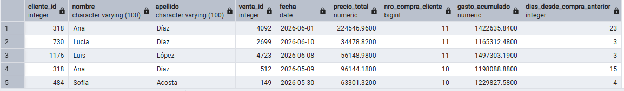
\includegraphics[width=1\linewidth]{image3.png}
    \caption{Resultado de la Consulta 1: top 3 productos más rentables dentro de cada categoría.}
\end{figure}

\subsubsection*{Consulta 2 — Comportamiento de compra de cada cliente en el tiempo}

\textbf{Para cada venta de un cliente identificado: ¿qué número de compra es, cuánto lleva
gastado acumulado y cuántos días pasaron desde su compra anterior?} Sirve para analizar la
recencia/frecuencia de compra de los clientes y así detectar clientes que dejan de comprar.

Utilizamos \textbf{función de ventana} porque las tres métricas dependen del \textbf{orden}
y la \textbf{posición} de cada compra dentro del historial del cliente, no globalmente:

\begin{itemize}[nosep]
    \item \texttt{ROW\_NUMBER() OVER (PARTITION BY cliente ORDER BY fecha)} $\rightarrow$
    número ordinal de compra.
    \item \texttt{SUM(precio\_total) OVER (PARTITION BY cliente ORDER BY fecha,hora,venta
    ROWS UNBOUNDED PRECEDING)} $\rightarrow$ \textbf{gasto acumulado}.
    \item \texttt{LAG(fecha) OVER (...)} $\rightarrow$ fecha de la compra anterior, para
    medir el intervalo entre compras.
\end{itemize}

\texttt{GROUP BY} no tiene concepto de «fila anterior» ni de orden: colapsaría todas las
compras del cliente en una sola fila y se perdería toda la secuencia temporal. Como
\texttt{precio\_total} ya no es columna de \texttt{VENTAS}, una CTE previa lo reconstruye
por venta ($SUM(cantidad \cdot precio\_unidad)$) y las funciones de ventana operan sobre
esa CTE.

\textbf{Resultado obtenido:}

\begin{figure}[ht]
    \centering
    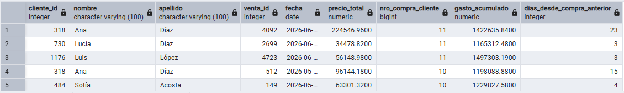
\includegraphics[width=1\linewidth]{image4.png}
    \caption{Resultado de la Consulta 2: número de compra, gasto acumulado y días desde la compra anterior por cliente.}
\end{figure}

\subsection{Funciones estadísticas}

Script: \textbf{\texttt{queries\_estadisticas.sql}}. Tabla analizada: \texttt{VENTAS}.
Como \texttt{VENTAS} ya no almacena columnas numéricas, las consultas que necesitan los
montos los reconstruyen por venta desde el detalle dentro de una CTE (\texttt{WITH}):
C1 arma una \texttt{ventas\_ext} completa (las 8 columnas), C2 una \texttt{ventas\_ext}
reducida con \texttt{precio\_total}/\texttt{costo\_total}, y C3 usa una CTE de conteo
(\texttt{conteo}) sobre \texttt{VENTAS} unida a \texttt{METODOS\_PAGO}. En los tres casos
se cumple el requisito de usar Common Table Expressions.

\subsubsection*{C1 — Perfil general de cada columna}

Para cada una de las 8 columnas de \texttt{ventas\_ext}: total de filas, filas no nulas,
\% no nulas y cantidad de valores distintos. Técnica: como cada columna tiene un tipo
distinto, se calcula el perfil por columna y se apilan con \texttt{UNION ALL} en formato
largo (una fila por columna). \texttt{COUNT(col)} ignora \texttt{NULL} mientras que
\texttt{COUNT(*)} cuenta todo: la diferencia revela los nulos (útil en
\texttt{cliente\_id}, la única columna nullable).
\begin{figure}[ht]
    \centering
    \includegraphics[width=0.6\linewidth]{consultaEst1.png}
    \caption{Perfil general de cada columna (C1): filas totales, no nulas y valores distintos.}
\end{figure}

\subsubsection*{C2 — Estadísticos de las columnas numéricas}

Para \texttt{precio\_total} y \texttt{costo\_total} (calculadas por venta): desvío
estándar, mínimo, \textbf{P05, Q1, mediana, promedio, Q3, P95}, máximo, cantidad y \% de
ceros, cantidad y \% de negativos, y \textbf{cantidad de outliers}. Técnicas destacadas:

\begin{itemize}[nosep]
    \item Las dos columnas numéricas (reconstruidas) se «despivotan» a formato largo con
    \texttt{UNION ALL} para calcular ambas en una sola pasada.
    \item Percentiles con \texttt{PERCENTILE\_CONT(p) WITHIN GROUP (ORDER BY valor)}
    (interpolados).
    \item Outliers por la \textbf{regla de Tukey}: fuera de
    $[Q1 - 1.5 \cdot IQR \; ; \; Q3 + 1.5 \cdot IQR]$, contados con
    \texttt{COUNT(*) FILTER (...)}.
\end{itemize}
\begin{figure}[ht]
    \centering
    \includegraphics[width=1\linewidth]{consultaEst2.png}
    \caption{Estadísticos de las columnas numéricas (C2): percentiles, dispersión y outliers.}
\end{figure}


\subsubsection*{C3 — Distribución de frecuencias de las columnas categóricas}

Para \texttt{metodo\_pago} y \texttt{puntos\_de\_venta\_id} (la sucursal, ya que
\texttt{estado\_entrega} fue eliminado): hasta los 10 valores más frecuentes con su
frecuencia y porcentaje, agrupando el resto en una fila (\texttt{resto}). Técnica: CTE de
conteo $\rightarrow$ \texttt{ROW\_NUMBER() OVER (ORDER BY frecuencia DESC)} para rankear
$+$ \texttt{SUM(frecuencia) OVER ()} para el total $\rightarrow$ \texttt{CASE} que separa
top 10 de (\texttt{resto}).

\begin{figure}[ht]
    \centering
    \includegraphics[width=0.5\linewidth]{consultaEst3.png}
    \caption{Distribución de frecuencias de las columnas categóricas (C3).}
\end{figure}

\subsection{Análisis de Performance}

Documento completo: \textbf{\texttt{Ejercicio\_2.3\_Analisis\_Performance.docx}}. Índice
propuesto: \textbf{\texttt{create\_index\_23.sql}}.

\subsubsection*{Consulta analizada}

Se eligió la \textbf{Consulta 1 de la Etapa 2.1} (ranking de productos más rentables por
categoría) por ser la más compleja: combina join de 3 tablas, \texttt{GROUP BY}, función
de ventana y dos ordenamientos. En el nuevo modelo \texttt{profit\_total} se calcula como
$SUM(cantidad \cdot (precio\_unidad - costo\_unidad))$ (las columnas
\texttt{subtotal}/\texttt{profit} ya no existen).

Todas las mediciones de costo y tiempo de esta sección se obtuvieron sobre
\textbf{PostgreSQL 16.4} (imagen \texttt{postgis/postgis:16-3.4}). Los costos y los planes
elegidos pueden variar entre versiones del motor (cambios en el optimizador) y entre
máquinas (los tiempos dependen del hardware y del estado de la caché).

\subsubsection*{Plan de ejecución original (EXPLAIN ANALYZE)}

\begin{figure}[ht]
    \centering
    \includegraphics[width=0.5\linewidth]{analyze1.png}
    \caption{Plan de ejecución original (\texttt{EXPLAIN ANALYZE}), sin índices adicionales.}
\end{figure}

Ejecutamos \texttt{EXPLAIN ANALYZE} sobre la consulta original (sin índices adicionales) y observamos la estructura del plan (de abajo hacia arriba). A diferencia de lo estimado en etapas tempranas con menos datos, el plan real con la base de datos poblada muestra lo siguiente:

\begin{table}[ht]
\centering
\caption{Costo acumulado por nodo del plan de ejecución original.}
\begin{tabular}{@{}lrr@{}}
\toprule
\textbf{Operación} & \textbf{Costo total acum.} & \textbf{Costo que agrega} \\
\midrule
Seq Scans sobre \texttt{detalle\_ventas}, \texttt{productos} y \texttt{categorias} & $\sim$241 & — \\
Hash Joins sucesivos para unir las 3 tablas & 332 & +91 \\
Sort (preparación para agrupar) & 1\,263 & +931 \\
GroupAggregate (el \texttt{GROUP BY}) & 1\,756 & +493 \\
Incremental Sort (ordenamiento para la ventana) & 2\,452 & +696 \\
WindowAgg (calcula \texttt{DENSE\_RANK}) & 2\,681 & +229 \\
Sort final por (\texttt{categoria}, \texttt{posicion\_en\_categoria}) & \textbf{5\,945} & +3\,264 \\
\bottomrule
\end{tabular}
\end{table}

\textbf{Lectura del plan:} La estructura revela que PostgreSQL optó por realizar escaneos secuenciales (\texttt{Seq Scan}) sobre las tres tablas. Como la consulta agrega toda la tabla \textbf{sin filtros WHERE}, el motor asume que leer las tablas completas para luego unirlas mediante \texttt{Hash Join} es la estrategia más económica. Gran parte del costo global reside en los nodos \textbf{Sort}, especialmente el ordenamiento final derivado de la función de ventana.

\subsubsection*{Solución propuesta y análisis comparativo}

Para mitigar el costo de lectura de la tabla de hechos (\texttt{detalle\_ventas}), que es la de mayor volumen, propusimos el siguiente índice cubriente:

\begin{lstlisting}[language=SQL]
CREATE INDEX idx_detalle_ventas_producto
ON detalle_ventas (product_id) INCLUDE (cantidad, precio_unidad, costo_unidad);
\end{lstlisting}

\textbf{Impacto tras aplicar el índice:}

\begin{figure}[ht]
    \centering
    \includegraphics[width=0.5\linewidth]{analyze2.png}
    \caption{Plan de ejecución tras crear el índice cubriente.}
\end{figure}

\begin{figure}[ht]
    \centering
    \includegraphics[width=1\linewidth]{analyze2 cerquita.png}
    \caption{Detalle del \texttt{Index Only Scan} sobre el índice cubriente (\texttt{Heap Fetches: 0}).}
\end{figure}

Al volver a ejecutar \texttt{EXPLAIN ANALYZE}, el plan de ejecución cambió drásticamente. El tiempo de ejecución real bajó de 20.45 ms a 14.37 ms y el costo bajó a 5844.

El optimizador abandonó el \texttt{Hash Join} sobre \texttt{detalle\_ventas}. En su lugar, utilizó un \texttt{Merge Join} entre categorías y productos, y un \texttt{Nested Loop} que se alimenta de un \textbf{Index Only Scan} sobre nuestro nuevo índice \texttt{idx\_detalle\_ventas\_producto}. 

El éxito de esta optimización radica en la cláusula \texttt{INCLUDE}: como el índice contiene las columnas base con las que la consulta calcula los \texttt{SUM} (\texttt{cantidad}, \texttt{precio\_unidad}, \texttt{costo\_unidad}), PostgreSQL resuelve la lectura sin necesidad de acceder a la tabla real en el disco (verificado por la métrica \texttt{Heap Fetches: 0}). Si bien la lectura de datos se optimizó al máximo logrando un escaneo exclusivo de índice, el costo global de la consulta sigue estando fuertemente dominado por los nodos \texttt{Sort} requeridos por \texttt{WindowAgg} y \texttt{GroupAggregate}.

% ============================================================================
\section{Etapa 3 — Procesamiento con Spark}
% ============================================================================

En esta etapa utilizaremos PySpark para procesar los datos y responder consultas con
MapReduce que serían muy difíciles o costosas de responder con un motor SQL convencional.
Implementaremos 3 procesamientos de MapReduce sobre datos del dominio.


\subsubsection*{Consulta 1 — Facturación, cantidad de ventas y ticket promedio por sucursal}

\textbf{Pregunta:} ¿cuánto facturó cada punto de venta y cuál es su ticket promedio?

\textbf{Map:} Unimos (join por \texttt{venta\_id}) el monto por venta con puntos de venta y
mapeamos (clave: \texttt{puntos\_de\_venta\_id}, valor: $(monto, 1)$).

\textbf{Reduce:} \texttt{reduceByKey} sumando las tuplas componente a componente por cada
punto de venta $\rightarrow$ $(suma\_facturacion, cantidad\_ventas)$. La operación es
asociativa y conmutativa, lo que habilita el \textit{map-side combine}. Un
\texttt{mapValues} final deriva el ticket promedio.

\textbf{Acción:} \texttt{collect()}.

\begin{figure}[ht]
    \centering
    \includegraphics[width=0.75\linewidth]{captura15.png}
    \caption{Facturación total, cantidad de ventas y ticket promedio por sucursal.}
\end{figure}

\subsubsection*{Consulta 2 — Top 10 productos por ganancia}

\textbf{Pregunta:} ¿cuáles son los 10 productos que más ganancias generaron? Esta pregunta
es similar a la primera consulta de la etapa 2 (ranking de productos más rentables por
categoría). Podemos ver que esta manera de resolverla es bastante más sencilla e intuitiva.

\textbf{Map:} por cada línea de \texttt{detalle\_ventas} mapeamos (clave:
\texttt{product\_id}, valor: $cantidad \cdot (precio\_unidad - costo\_unidad)$)
(calculamos la ganancia de cada venta de producto al mapear).

\textbf{Reduce:} reducimos por \texttt{product\_id} sumando la ganancia $\rightarrow$
ganancia total por producto.

\textbf{Acción:} \texttt{takeOrdered(10, key=-profit)}, que ordena de forma
\textbf{distribuida} (parcial por partición + combinación) sin traer todo el RDD al driver.

\begin{figure}[ht]
    \centering
    \includegraphics[width=0.5\linewidth]{captura16.png}
    \caption{Top 10 productos por ganancia total acumulada.}
\end{figure}

\subsubsection*{Consulta 3 — Distribución de ventas e ingresos por método de pago}

\textbf{Pregunta:} ¿cómo se reparten las ventas (cantidad y monto) entre los métodos de
pago?

\textbf{Map:} se \textbf{une} el monto por venta con \texttt{venta\_id} y mapeamos (clave:
\texttt{metodo\_pago}, valor: $(1, monto)$).

\textbf{Reduce:} \texttt{reduceByKey} sumando ambos componentes del valor
$(cantidad\_ventas, monto\_total)$ por método. Como hay solo 6 categorías, el shuffle es
mínimo.

\textbf{Acción:} \texttt{collect()}, y un paso final calcula el porcentaje sobre el total.

\begin{figure}[ht]
    \centering
    \includegraphics[width=0.6\linewidth]{captura17.png}
    \caption{Distribución de ventas e ingresos entre los métodos de pago.}
\end{figure}
% ============================================================================
\section{Etapa 4 — Persistencia Políglota (NoSQL)}
% ============================================================================

En este ítem, consideramos nuevos requerimientos hipotéticos del negocio que se verían
beneficiados por pasar a un paradigma de bases de datos NoSQL.

\subsection{Redis}

La carga de los datos, las consultas y las actualizaciones pedidas por el enunciado se
encuentran en el notebook: \textbf{\texttt{redis\_nosql.ipynb}}. Entorno: Redis 7.2 local
(Docker), \texttt{localhost:6379}, \texttt{decode\_responses=True}.

\subsubsection{Modelo Clave-Valor y Hashes}

Se modelan \textbf{tres} datos del dominio, que se ven beneficiados de utilizar la
estructura de Redis.

\begin{enumerate}[leftmargin=*]
    \item \textbf{Stock bidireccional (hashes espejo).} Dos hashes:
    \begin{itemize}[nosep]
        \item \texttt{stock:producto:<id>} con campos \texttt{sucursal\_id} $\rightarrow$ cantidad.
        \item \texttt{stock:sucursal:<id>} con campos \texttt{product\_id} $\rightarrow$ cantidad.
    \end{itemize}
    Duplicar el dato es \textbf{a propósito}: en Redis se modela según el patrón de acceso.
    Permite responder en \textbf{O(1)} «¿cuánto stock del producto P hay en la sucursal S?»
    con \texttt{HGET}, y también la dirección inversa. El precio a pagar (escribir en ambos
    hashes) son operaciones O(1) baratas. La \textbf{venta} descuenta stock con
    \texttt{HINCRBY} \textbf{atómico} sobre ambos hashes dentro de una transacción
    (\texttt{MULTI} vía pipeline) para que no se desfasen; luego se \textbf{verifica}
    releyendo las dos vistas. En este caso, Redis es ventajoso porque se puede consultar el
    stock para cierto producto en cierta sucursal en O(1), y con una latencia
    sub-milisegundo. Al ser un dato que interesaría consultar con mucha frecuencia, tiene
    sentido usar Redis.

    \item \textbf{Perfil de producto (hash).} \texttt{producto:<id>} con nombre, precio,
    marca. Se lee un campo (\texttt{HGET}) o el documento completo (\texttt{HGETALL}).
    \textbf{Actualización:} cambio de precio con \texttt{HSET} y verificación releyendo.
    Modelamos este dato usando Redis porque es información que suponemos que podría ser
    consultada con mucha frecuencia, y es un valor único para cada id (tipo de dato simple,
    fácil de implementar, mantener y consultar en Redis).

    \item \textbf{Contador de ventas del día (string).}
    \texttt{ventas:hoy:sucursal:<id>} con \texttt{INCR} atómico y
    \texttt{caja:sucursal:<id>} con \texttt{INCRBYFLOAT}. Utilizamos Redis en este caso
    porque es un dato que se actualizaría frecuentemente, y Redis permite la actualización
    atómica con \texttt{INCR}/\texttt{HINCRBY} por diseño.
\end{enumerate}

\subsubsection{Lista como cola de pedidos (nuevo requerimiento: ventas online con envío)}

Supongamos que el negocio decide incorporar \textbf{venta online con envío}: el pedido no
se entrega en el acto, queda \textbf{pendiente de despacho}. Se modela una \textbf{cola
FIFO} con una lista de Redis (\texttt{pedidos:pendientes}):

\begin{itemize}[nosep]
    \item \textbf{Al concretarse una venta} $\rightarrow$ \texttt{RPUSH} (entra por el final).
    \item \textbf{Al despachar} $\rightarrow$ \texttt{LPOP} (sale el más antiguo, del frente).
\end{itemize}

\texttt{RPUSH} + \texttt{LPOP} implementan FIFO. Cada pedido se serializa como JSON.
Operaciones mostradas:

\begin{itemize}[nosep]
    \item \textbf{Consulta:} \texttt{LRANGE} (ver la cola sin modificarla), \texttt{LLEN}
    (tamaño), \texttt{LINDEX 0} (peek del próximo a despachar).
    \item \textbf{Gestión:} \texttt{LPOP} (despachar), \texttt{RPUSH} (encolar nuevo),
    \texttt{RPOP} (cancelar el último ingresado).
    \item \textbf{Simulación del flujo completo:} se intercalan ventas y despachos
    mostrando cómo crece y se vacía la cola en cada paso.
\end{itemize}

\subsubsection{TTL — Datos con tiempo de vida}

Implementamos tres datos con tiempo de vida. La siguiente tabla indica los datos, el
tiempo de vida elegido, y la justificación.

\begin{table}[ht]
\centering
\caption{Datos con TTL en Redis: clave, tiempo de vida y justificación.}
\renewcommand{\arraystretch}{1.5}
\begin{tabular}{@{}p{2.6cm}p{5.3cm}p{1.3cm}p{6cm}@{}}
\toprule
\textbf{Dato} & \textbf{Clave} & \textbf{TTL} & \textbf{Por qué ese tiempo} \\
\midrule
Carrito de compras & \texttt{carrito:cliente:<id>} & 30 min &
Conserva la selección mientras el cliente compra; libera carritos abandonados. Se
\textbf{renueva} con \texttt{EXPIRE} en cada acción. \\
Reserva temporal de stock & \texttt{reserva:stock:<prod>:<suc>} & 10 min &
Reserva unidades mientras el cliente paga; si no concreta, el stock se libera (evita
sobreventa sin congelar inventario). \\
Token de sesión & \texttt{sesion:token:<token>} & 1 hora &
Mantiene logueado al cliente; vence por seguridad ante inactividad. \\
\bottomrule
\end{tabular}
\end{table}

\subsection{MongoDB}

Notebook: \textbf{\texttt{mongodb\_documental.ipynb}}. Configuración del entorno disponible
en \texttt{readme.md}.

\subsubsection{Diseño de colecciones}

Para este apartado, suponemos que el negocio quiere empezar a vender productos en combos.
Incluir esto en el modelo relacional provocaría que cada línea de \texttt{DETALLE\_VENTAS}
haga referencia o bien a un producto, o bien a un combo. Es decir, \texttt{DETALLE\_VENTAS}
tendría a la vez \texttt{product\_id} y \texttt{combo\_id}, como clave foránea, manteniendo
siempre uno en \texttt{NULL} por fila más un \texttt{CHECK} que garantice que exactamente
uno esté presente. En el modelo documental esto se puede reproducir de la siguiente forma,
evitando el desperdicio de espacio.

Modelamos dos colecciones:

\begin{itemize}[leftmargin=*]
    \item \textbf{ventas} — consiste en un documento por operación que integra la
    información de la transacción y sus ítems embebidos en el \textit{array}
    \texttt{items[]}. Cada elemento del \textit{array} se clasifica como
    \texttt{tipo:"producto"} o \texttt{tipo:"combo"} e incluye un ID referencial
    \texttt{producto\_id} o \texttt{combo\_id} según corresponda, junto a otros datos
    pertinentes. A su vez, la venta también contiene datos referenciales a otras entidades
    como \texttt{cliente\_id} y \texttt{punto\_de\_venta\_id}.
    \item \textbf{combos} — en esta colección cada documento representa un combo, teniendo
    datos del mismo y los productos que lo componen en un \textit{array} embebido
    \texttt{componentes[]}. Este \textit{array} contiene el ID referencial
    \texttt{producto\_id} y su cantidad.
\end{itemize}

\paragraph{Decisiones de diseño discutidas:}
\begin{itemize}[leftmargin=*]
    \item \textbf{Embeber vs. referenciar:} se decidieron embeber las líneas de ventas y
    los componentes de los combos debido a que se suelen leer y escribir juntos (pueden
    verse como entidades débiles). En ventas, se hace referencia al cliente y al punto de
    venta porque son entidades completamente distintas con relación uno a muchos; por otro
    lado, \texttt{combo\_id} y \texttt{producto\_id} se guardan como referencia para saber
    qué producto se vendió, pero también estos atributos se encuentran embebidos junto a
    una copia del precio y demás datos al momento de la venta para mantener una facturación
    histórica.
    \item \textbf{Campos opcionales:} existen campos opcionales como \texttt{cliente\_id}
    (podrían registrarse ventas anónimas) o descripción de combo (la cual es opcional).
    Además, los campos en \texttt{items[]} varían según el tipo (un ítem-combo tiene
    \texttt{combo\_id}; un ítem-producto tiene \texttt{producto\_id}).
    \item \textbf{Diferencia con el relacional:} en este caso, no resulta necesaria la
    tabla \texttt{DETALLE\_VENTAS}, ni la implementación de FKs con \texttt{CHECK} de
    exclusividad.
\end{itemize}

Se \textbf{generaron} \textbf{100} documentos \textbf{combos} y \textbf{130} documentos
\textbf{ventas}, con variedad (sólo productos, productos y combos, con y sin cliente,
distintos métodos de pago, fechas en 6 meses; combos con y sin descripción).

\subsubsection{Operaciones CRUD}

Cada operación atada a un caso de uso:

\begin{itemize}[leftmargin=*]
    \item \textbf{Inserción (\texttt{insert\_one} / \texttt{insert\_many}):} se insertan
    los documentos generados en 4.2.1. Se usa \texttt{insert\_one} para el primer documento
    e \texttt{insert\_many} para el resto.
    \item \textbf{Read con filtros:} se buscan las ventas entre \$40.000 y \$120.000 pagadas
    con tarjeta o MercadoPago, utilizamos \texttt{\$gte}, \texttt{\$lte}, \texttt{\$or} y
    \texttt{\$and}.
    \item \textbf{Proyección:} un listado de \texttt{fecha}, \texttt{precio\_total},
    \texttt{metodo\_pago} para un reporte, se oculta \texttt{\_id} y el array
    \texttt{items}.
    \item \textbf{Update:} se realizaron 3 operaciones con \texttt{\$set}, \texttt{\$inc},
    \texttt{\$push}; dar de baja un combo (\texttt{\$set activo=false}); aumentar \$500 el
    precio de todos los combos (\texttt{\$inc} + \texttt{update\_many}); agregar un ítem a
    una venta (\texttt{\$push}) y ajustar su total (\texttt{\$inc}).
    \item \textbf{Delete:} se insertan documentos de prueba marcados y luego se borran con
    \texttt{delete\_one} y \texttt{delete\_many}.
\end{itemize}

\subsubsection{Aggregation Pipelines}

\paragraph{Pipeline A — Top 5 combos más vendidos.} ¿Qué combos facturan más y cuál es su
composición?

\begin{enumerate}[nosep]
    \item \texttt{\$unwind items} $\rightarrow$ devuelve los items de las ventas.
    \item \texttt{\$match tipo = "combo"} $\rightarrow$ filtra los ítems-combo.
    \item \texttt{\$group} por \texttt{combo\_id} $\rightarrow$ agrupa por \texttt{\_id},
    suma subtotal y cantidad, resultando en facturación y unidades respectivamente.
    \item \texttt{\$sort} por facturación descendiente, con \texttt{\$limit = 5}.
    \item \texttt{\$lookup} a combos $\rightarrow$ obtiene nombres y componentes del catálogo.
    \item \texttt{\$unwind} + \texttt{\$project} $\rightarrow$ forma de salida (incluye
    \texttt{\$size} de componentes).
\end{enumerate}

\begin{figure}[ht]
    \centering
    \includegraphics[width=0.75\linewidth]{pipelineAMongoDB.png}
    \caption{Pipeline A: top 5 combos más vendidos y su composición.}
\end{figure}

\paragraph{Pipeline B — Facturación total y valor de tickets promedio por mes.} ¿Cómo
evoluciona la facturación mes a mes?

\begin{enumerate}[nosep]
    \item \texttt{\$group} por año-mes de \texttt{fecha} $\rightarrow$ total facturado
    (\texttt{\$sum precio\_total}), ticket promedio (\texttt{\$avg precio\_total}) y
    cantidad de ventas (\texttt{\$sum 1}).
    \item \texttt{\$sort} cronológico.
    \item \texttt{\$project} $\rightarrow$ etiqueta YYYY-MM legible del periodo,
    facturación, ventas y ticket promedio.
\end{enumerate}

\begin{figure}[ht]
    \centering
    \includegraphics[width=0.65\linewidth]{pipelineBMongoDB.png}
    \caption{Pipeline B: facturación total y ticket promedio mes a mes.}
\end{figure}

\subsubsection*{Reflexión: PostgreSQL vs. MongoDB}

Concluimos que MongoDB es más natural en el caso de Combos y Ventas. En primer lugar,
porque cada ítem producto o combo se modela con documentos polimórficos; en SQL requería
dos FKs (una siempre \texttt{NULL}) + \texttt{CHECK} + tabla \texttt{COMBOS} y tabla
\texttt{CONTIENE}. Además, permite la lectura de la venta completa sin utilizar joins: cada
venta es un documento independiente del resto de las colecciones.

Por otro lado, concluimos que la principal desventaja que tiene MongoDB frente a PostgreSQL
es la desnormalización. En primer lugar, la independencia entre colecciones pone en peligro
la consistencia: por ejemplo, podrían aparecer combos en ventas que no existen en la
colección de Combos; esto debería manejarse durante el mantenimiento, asegurándose que al
registrar una nueva venta, el combo exista en la tabla combos. Sin embargo, como la tabla
ventas funciona como un registro histórico, no hay costos de mantenimiento extras por
actualizaciones: es decir, si se produjera un cambio en un combo, no habría que recorrer
toda la colección de ventas y actualizar, en cada venta, ese combo. Esto produce que, para
los datos modelados, el enfoque documental resulte beneficioso.
\section{Reflexión final: PostgreSQL vs. MongoDB vs. Spark}

El desarrollo de este trabajo demuestra que no existe una base de datos "bala de plata"; la arquitectura políglota es la respuesta a las demandas modernas.

\begin{itemize}
    \item \textbf{PostgreSQL} brilla como fuente de verdad transaccional (ACID) y es imbatible para cálculos analíticos complejos sobre relaciones estrictas (rankings, funciones de ventana y agregaciones con múltiples joins), aprovechando sus índices y su optimizador maduro.
    \item \textbf{MongoDB} resulta mucho más natural y eficiente para entidades heterogéneas o con esquemas variables, como el caso de las Ventas y Combos. Al embeber las líneas de detalle dentro de un único documento polimórfico, se evitan \texttt{JOINs} costosos y columnas nulas (\texttt{NULLs} dispersos): la transacción completa se recupera con una sola lectura del documento, en lugar de reconstruirla uniendo varias tablas. Sin embargo, su debilidad recae en la responsabilidad que delega a la aplicación para mantener la consistencia de los datos ante actualizaciones de catálogo. Por eso \textbf{no resulta conveniente} cuando se necesita integridad referencial fuerte, transacciones ACID multi-documento o reportes analíticos con agregaciones y joins arbitrarios entre muchas entidades: en esos escenarios PostgreSQL sigue siendo la mejor opción.
    \item \textbf{Apache Spark}, por su parte, entra en juego donde los motores relacionales convencionales se ahogan: el volumen masivo distribuido. Mientras que Postgres o Mongo procesan datos en una única instancia (o réplicas), el modelo de evaluación perezosa y el motor in-memory de Spark le permiten barrer millones de registros y realizar operaciones de agregación (MapReduce sobre RDDs) distribuyendo la carga a través de múltiples nodos de forma nativa.
\end{itemize}

\textbf{Conclusión:} La persistencia políglota consiste en usar cada herramienta donde es fuerte. PostgreSQL para integridad relacional, facturación estricta y analítica con joins y funciones de ventana; Redis para baja latencia en estados efímeros (colas, carritos y TTL); MongoDB para catálogos ricos y transacciones anidadas con esquema variable; y Spark para analítica distribuida a gran escala.
% ============================================================================
\section*{Anexo — Índice de archivos del repositorio}
\addcontentsline{toc}{section}{Anexo — Índice de archivos del repositorio}
% ============================================================================

\begin{longtable}{@{}p{8cm}p{1.4cm}p{8cm}@{}}
\caption{Índice de archivos del repositorio.}\\
\toprule
\textbf{Archivo} & \textbf{Etapa} & \textbf{Contenido} \\
\midrule
\endhead
\texttt{creacion\_tablas.sql}                    & 1.2 & Esquema: tablas, PK, FK, constraints \\
\texttt{generar\_datos.py}                       & 1.3 & Generador reproducible $\rightarrow$ \texttt{poblado\_datos.sql} \\
\texttt{poblado\_datos.sql}                       & 1.3 & INSERTs (> 5000 registros principales) \\
\texttt{validar\_datos.sql}                       & 1.3 & Validaciones de consistencia + estadísticos \\
\texttt{der.drawio} / \texttt{der.png}            & 1.1 & Diagrama Entidad-Relación \\
\texttt{queries\_con\_funciones\_ventana.sql}     & 2.1 & 2 consultas con funciones de ventana \\
\texttt{queries\_estadisticas.sql}                & 2.2 & C1/C2/C3 con CTE \\
\texttt{Ejercicio\_2.3\_Analisis\_Performance.docx} & 2.3 & Análisis de EXPLAIN \\
\texttt{create\_index\_23.sql}                    & 2.3 & Índice propuesto \\
\texttt{mapreduce\_spark.ipynb}                   & 3.1 & 3 MapReduce con RDDs \\
\texttt{redis\_nosql.ipynb}                       & 4.1 & KV/hashes, listas/cola, TTL \\
\texttt{mongodb\_documental.ipynb}                & 4.2 & Diseño documental, CRUD, aggregation \\
\texttt{README.md}                                & — & Instrucciones de reproducción \\
\bottomrule
\end{longtable}

\end{document}
